% !TeX root = ../tesis.tex

% -----------------------------------------------------------------------
\section{El Anillo Periférico: Un Proyecto Político Estructural}
\label{sec:anillo-periferico}
% -----------------------------------------------------------------------

La construcción del Anillo Periférico, junto con el Viaducto Miguel Alemán, debe
analizarse no como una simple necesidad de infraestructura, sino como la
expresión
material y simbólica de la hegemonía de la automovilidad como política de Estado
durante la regencia de Ernesto P. Uruchurtu (1952--1966) \citep{franco2022}.
La magnitud de estas obras subraya el giro drástico que la administración de
Ruiz
Cortines imprimió a la agenda de gobierno para el Distrito Federal, requiriendo
un
funcionario con la energía y la afinidad ideológica de Uruchurtu, cuya
trayectoria
previa le había proporcionado un conocimiento directo de la función
administrativa
del \textsc{ddf} \citep[Tomo~1, p.~173]{perlo2023}.

% -----------------------------------------------------------------------
\subsection{Centralización Administrativa y la Creación de los XII Cuarteles}
\label{subsec:xii-cuarteles}
% -----------------------------------------------------------------------

Antes de la ejecución de la mega-obra vial, la regencia de Uruchurtu se enfocó
en
la reestructuración administrativa y financiera del Departamento del Distrito
Federal
(\textsc{ddf}). Esta etapa inicial (1952--1953) incluyó una reforma a la
recaudación
de impuestos que generó un aumento sustancial del presupuesto para obra pública,
lo cual sentó las bases para el posterior desarrollo urbano.

Derivado de este crecimiento poblacional y la necesidad de optimizar la
prestación
de servicios, el regente procedió a la división del \textsc{ddf} en doce
Cuarteles.
Según la documentación, esta delimitación fue estrictamente administrativa y de
vigilancia, sin peso político-estatal directo, orientada a un control
poblacional y
estratégico de la Ciudad de México. No obstante, el alcance de esta estrategia
fue
rápidamente superado por la expansión física de la mancha urbana que forjó la
naciente Área Metropolitana de la Ciudad de México.

La importancia de esta división radica en su impacto urbanístico posterior: el
diseño
del Anillo Periférico y el Circuito Interior representó la materialización
geográfica
de los límites de estos Cuarteles \citep[Tomo~1, p.~257]{perlo2023}. Esta
correlación entre el límite administrativo de control y la infraestructura vial
más
ambiciosa de la época permite afirmar que la creación de ambos circuitos fungió
como
una delimitación operativa y simbólica que, si bien fue superada en su función
de
control, sigue siendo una referencia fundamental en la división económica y
política
de la capital.

\begin{figure}[H]
    \centering
    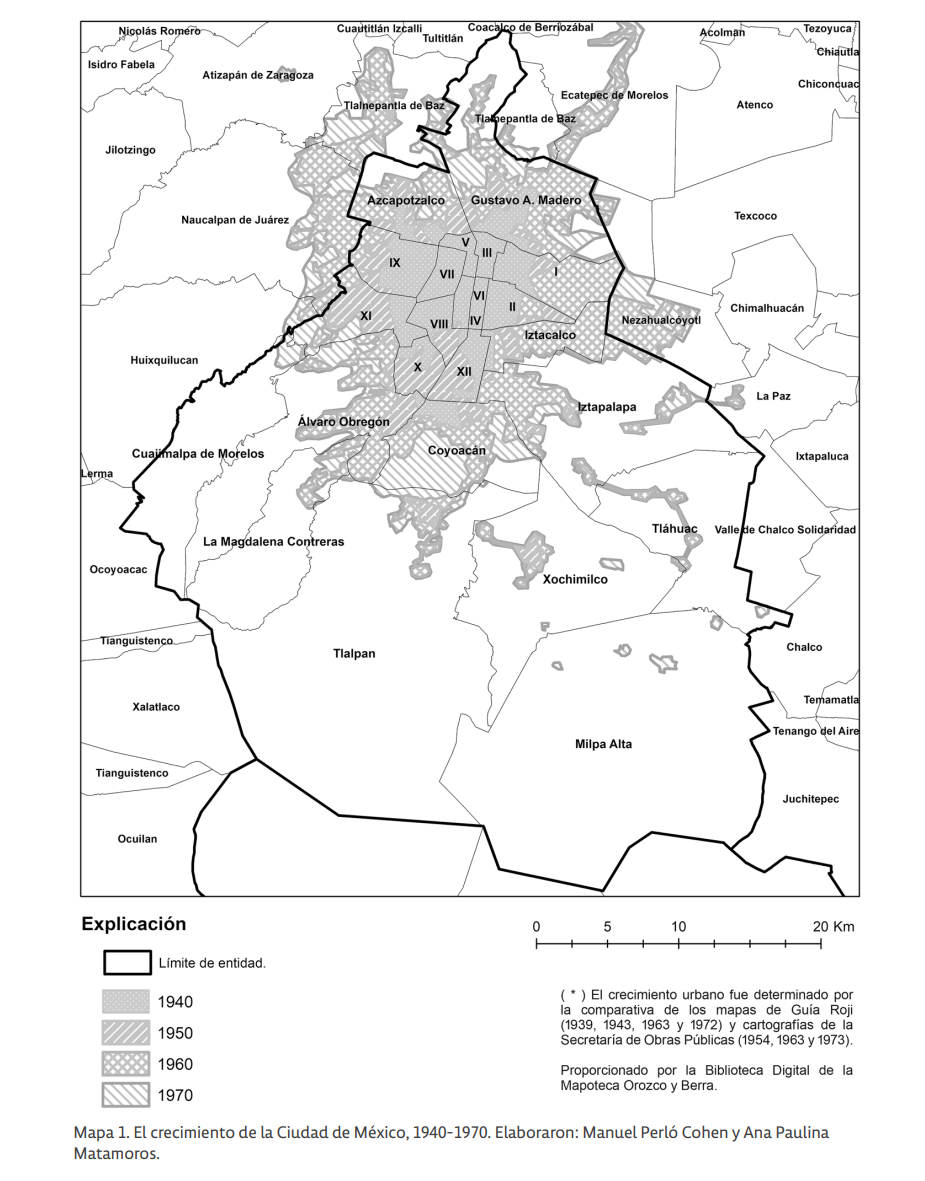
\includegraphics[width=0.82\textwidth]{Figures/Cap1/Uruchurtu1}
    \caption[Designación de los XII Cuarteles en la Ciudad de México]{Designación
de los XII Cuarteles en la Ciudad de México y crecimiento de la mancha urbana
    (1940--1970).}
    \label{fig:xii-cuarteles}
    \fuentefigura{Perlo Cohen (2023, p.~257).}
\end{figure}

% -----------------------------------------------------------------------
\subsection{La Prioridad Presupuestal: El Sesgo Vial Hegemónico}
\label{subsec:sesgo-vial}
% -----------------------------------------------------------------------

La materialización de la modernidad urbana, bajo la óptica de Uruchurtu, se basó
en
la implementación de grandes avenidas y vías rápidas orientadas exclusivamente
al
automóvil. Entre las obras más destacadas se encuentran el Viaducto Miguel
Alemán,
la Avenida Río Churubusco, el Circuito Interior y el Anillo Periférico. Este
último,
que se extendía desde Cuatro Caminos hasta Cuemanco, se concibió como la
principal arteria de comunicación, representando una obra moderna y cosmopolita
destinada a servir al flujo vehicular masivo.

La decisión de priorizar estas obras no fue una casualidad de la planeación,
sino un
sesgo presupuestal deliberado. \citet[Tomo~1, p.~391]{perlo2023} documenta
que
solo en 1958, el \textsc{ddf} destinó \$408 millones de pesos a obras en
avenidas,
banquetas, pavimentos y pasos a desnivel. Esta inversión superó con creces la
suma
destinada a servicios sociales esenciales como mercados, escuelas y centros
asistenciales, evidenciando que la eficiencia del flujo vehicular era el
criterio rector
del desarrollo urbano por encima de la equidad social o la integración
territorial.

% -----------------------------------------------------------------------
\subsection{El Déficit Estructural y el Rechazo al Metro}
\label{subsec:rechazo-metro}
% -----------------------------------------------------------------------

A pesar de la magnitud de la inversión vial, el \textsc{ddf} afrontaba una
crisis de
movilidad imposible de ignorar. Para finales de la década de 1950, la mayoría de
la
población carecía de automóvil propio, dependiendo de un sistema de autobuses de
rutas concesionadas caracterizado por ser precario e ineficiente. La respuesta
del
gobierno se limitó a la ampliación de rutas y a la promoción de transportes
eléctricos
(trolebuses y tranvías), una estrategia insuficiente ante el crecimiento
desmedido
de la urbe.

El punto de inflexión que definió el futuro de la movilidad capitalina fue el
rechazo
de Uruchurtu a la propuesta de un tren subterráneo ---el actual Sistema de
Transporte
Colectivo Metro---, presentada por el ingeniero Bernardo Quintana Arrioja a
principios
de la década de 1960. El regente desestimó la idea por considerarla costosa,
invasiva e innecesaria, argumentando la supuesta inviabilidad del proyecto
debido al
suelo fangoso de la ciudad. Esta decisión tuvo un impacto trascendental,
retrasando
la construcción del Metro hasta 1967 y consolidando el predominio del transporte
superficial y motorizado.

En síntesis, las obras de Uruchurtu carecieron de un programa articulado y
basado
en un patrón urbanístico refinado, respondiendo principalmente a las necesidades
inmediatas que el regente logró identificar. El legado del Periférico es una
fragmentación funcional: internamente, delimitó el orden administrativo de los
XII
Cuarteles; externamente, propició un crecimiento sin orden que ha dejado a los
territorios periféricos sin conectividad de transporte masivo hasta el día de
hoy.

